\documentclass[14pt]{matmex-diploma-custom}
\linespread{1.5}
\usepackage{listings}
\usepackage{cite}

\usepackage{framed}
\usepackage{tikz}
\usetikzlibrary{arrows}
\usepackage{amssymb}
\newcommand{\cd}[1]{\texttt{#1}}
\usepackage[caption=false]{subfig}
\usepackage{lstcoq}
\graphicspath{{images/}}%путь к рисункам

%\lstdefinelanguage{haskell}{
%keywords={data, type, case, of, where, otherwise, in, let, deriving},
%sensitive=true,
%basicstyle=\small,
%commentstyle=\scriptsize\rmfamily,
%keywordstyle=\ttfamily\underbar,
%identifierstyle=\ttfamily,
%basewidth={0.5em,0.5em},
%columns=fixed,
%fontadjust=true,
%literate={->}{{$\to$}}1
%}

\lstset{
basicstyle=\small,
identifierstyle=\ttfamily,
keywordstyle=\bfseries,
commentstyle=\scriptsize\rmfamily,
basewidth={0.5em,0.5em},
fontadjust=true,
escapechar=~,
language=haskell
}
%\DeclareMathSizes{16}{16}{16}{16}
\definecolor{dkviolet}{RGB}{100,0,100}
\definecolor{ltblue}{RGB}{0,100,100}
\definecolor{dkblue}{RGB}{0,50,50}

\begin{document}

\filltitle{ru}{
    chair              = {Кафедра Системного Программирования},
    title              = {История языков ML},
    author             = {ИЗМЕНИТЬ ИЗМЕНИТЬ ИЗМЕНИТЬ },
    supervisorPosition = {к.\,ф.-м.\,н.},
    supervisor         = {Терехов А.\,Н.},
}
\sloppy

\maketitle
\tableofcontents

\newpage
\section{Введение}
В попытке классифицировать языки программирования можно выделить два типа: декларативные и императивные. Современные императивные языки однозначно классифицировать не так просто, потому что почти все успешные языки сочетают в себе особенности различных стилей программирования. Например: объектно-ориентированный подход; поддержка функций как сущностей первого порядка; поддержка встроенных языков, специфичных для конкретной предметной области, и т.д. Однако, если у $C\!+\!+$ и $Java$ искать общего предшественника, то в нём инструкции должны выполняться последовательно друг за другом и должна быть поддержка изменяемых значений. Именно языки с такими свойствами принято называть императивными.

Своей популярности императивное программирование обязано в первую очередь устройству современного компьютера. Язык $C$ предоставляет прямой доступ к памяти и регистрам современных процессоров, позволяя писать максимально эффективный код под данную архитектуру. Однако, программисту на $C$ приходится самостоятельно беспокоиться о правильном выделении памяти и о корректном доступе к ней. В программах на $C$ большинство низкоуровневых особенностей компьютера на виду, а компиляторы $C$ не позволяют находить ошибки доступа к памяти или позволять программисту использовать высокий уровень абстракции. Поэтому язык $C$ считается языком низкого уровня.

Идейные наследники языка $C$ (например, $C\!+\!+$ или $Java$) позволяют программисту меньше беспокоиться об управлении памятью и писать программы на более высоком уровне абстракции. Однако, из-за удаления языка от архитектуры компьютера программы на высокоуровневых языках в ограничены по производительности. При этом современные языки программирования унаследовали концепцию изменяемых переменных, а она очень сильно осложняет создание формальной семантики языков программирования, а этот вопрос в последнее время приобретает всё большую популярность. Изменяемые значения также осложняет статическое исследование программ: поведение кода зависит не только от него самого, но и от всего окружения, в котором он выполняется.

Во второй половине ХХго века также велись исследования в области функциональных языков программирования: языков, в которых абстракция достигается с помощью использования функций, и вопрос необходимости использования изменяемого состояния стоит не так остро. Все они основаны на $\lambda$-исчислении Алонзо Чёрча (Alonzo Church), для некоторых построены формальные модели, другие основаны на формальных математических моделях. Долгое время они находились в тени императивных языков программирования, потому что для эффективной работы с ними требуется наличие автоматического управления памятью, что сказывается на эффективности программ. Долгое время функциональные языки компилировались в код на языке $LISP$, который интерпретировался, при этом весьма медленно. С ростом производительности и объёмов памяти у компьютеров функциональные языки получили возможность соревноваться по производительности с императивными языками, а современные императивные языки начали перенимать языковые конструкции, характерные для функционального программирования.

Целью данного реферата является рассмотрение пути развития наиболее известного статически типизируемого языка $M\!L$, а также родственных с ним языков. Будут рассмотрены работы учёных, которые оказали на его развитие наибольшее влияние, а также найден общий предок $M\!L$ и современных императивных языков программирования. Кроме этого, будут рассмотрены причины и контекст, в которых эти языки появились. Будут указаны ошибки при развитии языков, а также подчеркнуты цели, к которым стоит стремиться при разработке нового языка программирования.


\begin{center}
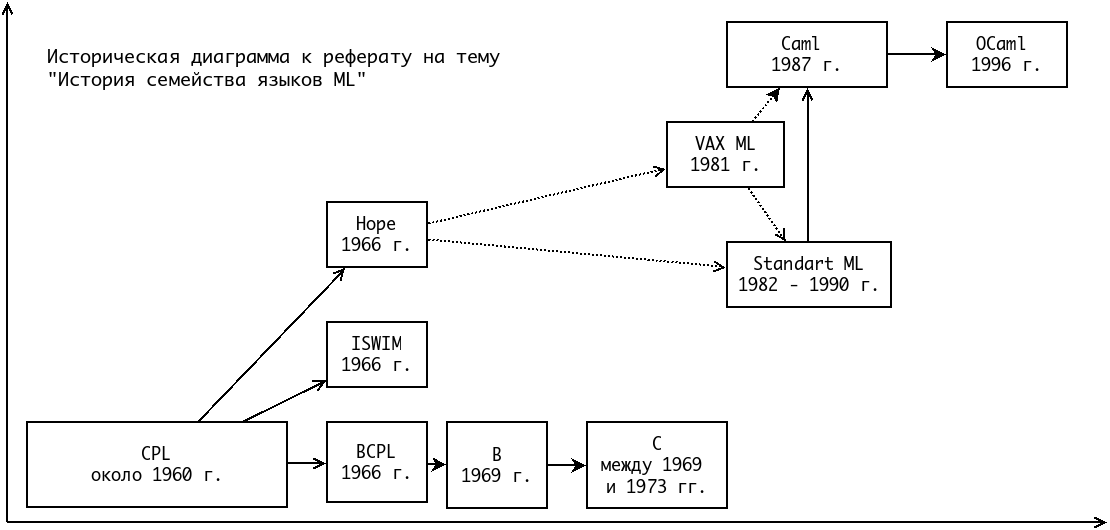
\includegraphics[angle=90,scale=0.585]{Diagram.png}
\end{center}

\section{Предыстория развития ML в Британии}
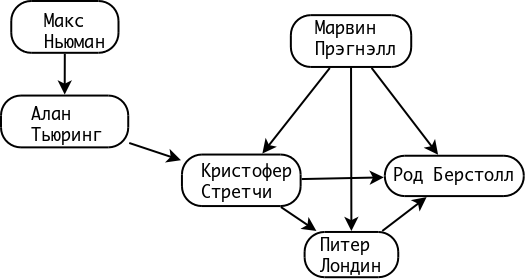
\includegraphics[angle=0,scale=0.4]{british.png}

Говоря об основоположниках $M\!L$ стоит упомянуть таких британских ученых как Макс Ньюман (Max Newman), Алан Тьюринг (Alan Turing), Кристофер Стрэйчи (Cristopher Strachey), Петер Лондин (Peter Laundin), Род Бeрстолл (Rod Berstall) и Марвин Прэгнелл (Marvin Pragnell). Среди них идейным лидером можно назвать Кристофера Стрейчи, а Марвина Прэгнелла -- "катализатором". Однажды, Марвин Прэгнелл увидел в кафе человека, который читает книгу Principia Mathematica \cite{russel1} и пригласил его на семинар, этим человеком оказался Питер Лондин. С Родом Берстоллом случилась аналогичная история, но в библиотеке. Сам семинар проводился в колледже Бёркберк без разрешения руководителей колледжа. Марвин Прэгнелл нашел человека с ключом, который их впустит аудиторию, где они заседали до позднего вечера. Вместе с Кристофером Стрэйчи, Петером Лондиным и Родом Берстолом семинар несколько раз посещал и Робин Милнер. Там они обсуждали вопросы логики, теории категорий и компьютеров. Вероятно, с этого любительского семинара и стоит отсчитывать историю ML. Случайные посетили вспоминали, что на нём всё было устроено несколько по-любительски, в отличие от того как такие вещи были организованы в США. При этом стоит заметить, что участники не являлись формально учеными, а были работающими программистами.

\subsection{Кристофер Стрейчи}
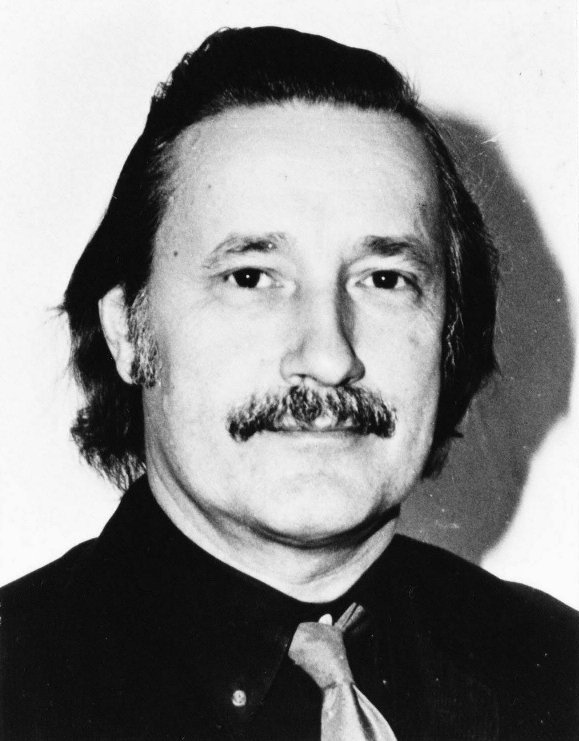
\includegraphics[angle=0,scale=0.2]{stratchey.jpg}

Кристофер Стрейчи (Cristopher Stratchey, 1916-1975) был другом Алана Тьюринга, когда тот работал в Кембридже и Манчестере. Он известен тем, что написал программу для игры в шашки в 1951 году в Национальной Физической Лаборатории (National Physical Laboratory, NPL). Это, возможно, была первая играющая программа для компьютера. Эта программа запускалась на машине Марк-1 манчестерского университета, так как эта машина имела намного больше памяти чем, например, машина $ACE$, которую спроектировал Алан Тьюринг. Для Марк-1 Кристофер Стрэйчи также написал первую программу для проигрывания простых мелодий, а именно детской песенки $Baa\ Baa\ Black\ Sheep$.

Что касается языков программирования, Кристофер Стрейчи спроектировал $C\!PL$ ($Combined\ Programming\ Language$), который назывался изначально 
$Cambridge\ Programming\ language$, а после переезда в Лондон был переименован в $Combined$. Также его называли в шутку $Cristopher’s\ programming\ language$. В этом языке были функции как сущности первого класса, а также было впервые введено понятие L-values --- выражений, которые вычисляются в место, где они хранятся. $CPL$ никогда не был успешно реализован, были прототипы и в Лондоне, и в Кембридже, но язык был очень амбициозен и сложен для того времени, так что его компиляторы никогда не появились и пользователей у него не было. Однако, Мартин Ричардс написал выпускную работу про компилятор этого языка, и вскоре решил, что было бы хорошо несколько упростить язык $CPL$. Так появился $Basic\ CPL$ ($BCPL$)\cite{bcpl1}, компилятор которого был реализован. Это был очень успешный язык для реализации больших систем в конце 60х -- начале 70х, который использовался, например, в компании Xerox Park. А в Bell Labs Кен Томпсон (Kenneth Thompson) также начал использовать его и улучшать. Так появился язык $B$, который потом эволюционировал в $C\!+\!+$.

\begin{verbatim}
CPL  =>  BCPL  =>  B  =>  C  =>  C++
\end{verbatim}

Также Кристофер Стрэйчи ввёл понятие каррирования (currying). В середине 1960х он написал очень важную работу, представленную на конференции в Копенгагене в 1967, которая называлась  “Фундаментальные понятия в языках программирования“ \cite{strachey1}. В ней он описывал различные виды полиморфизма и первым описал параметрический полиморфизм. Так же он известен как создатель денотационной семантики Скотта-Стрейчи (совместно с Дана Скотт (Dana Scott) в 1969 \cite{scott1}, который предоставил математическое обоснование этой семантики, основанной на лямбда-исчислении). Также Кристофер Стрейчи первым дал формальное определение продолжений (continuations). Он пришел к идее разделения времени (time-sharing, 1958, \cite{strachey2}) правда в несколько урезанном виде. В 1960-64 годах он нанял Питера Лондина (Peter Lundin) как своего помощника, который работал в национальной Лаборатории физики и в National Research and Develpment Corporation в Лондоне, а с 1959 Питер Лондин стал работать как независимый консультант. 

\begin{framed}
Вот что пишет ученик Стрейчи Крис Водсворт:

“К.Стрейчи имел особое чутьё в тех случаях, когда что-то было сделано “правильно” -- в основном когда было достаточно просто и достаточно элегантно, что выглядеть интуитивно правильным -- и он презирал чересчур проработанные и умудренные методы которые “кое-как работали”. Его любимым принципом был такой: “Ты можешь затолкать на гору горошину носом, но это не будет являться правильным способом осуществления этого”. Я это называл “тестом Стрейчи”.”
\end{framed}
%\begin{framed}
%Бёрнсталл о Стретчи
%His elegance of Manor was accompanied by an elegance of thought and language which was a continual inspiration.
%\end{framed}

\subsection{Питер Лондин}
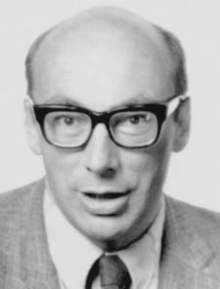
\includegraphics[angle=0,scale=0.585]{220px-Peter_Landin.png}

Питер Лондин (Peter Landin) написал множество статей в 1960х годах.

В статье “Механическое вычисление выражений”\cite{laundin1} он ввел понятие SECD-машины. Это не была первая абстрактная машина в мире, он использовал идеи сообщества программистов на языке $ALGOL$ из города Мюнхен. 

В статье "Соответсвие между языком $ALGOL60$ и лямбда-нотацией Чёрча: части 1 и 2"\cite{laundin2} он ввел понятие потоков (streams), которые являются особого рода методом для осуществления ввода-вывода.

В статье "Обобщение переходов и меток" \cite{laundin3} он ввел понятие $J$-оператора, который является предшественником термина продолжение (continuation).

Статья "The next 700 programming languages" \cite{laundin4} 1966 года описывает $I\!SW\!I\!M$ язык, который оказал влияние на $M\!L$.

В соавторстве с Родом Берстоллом в 1969 году была опубликована статья \cite{laundin5}, в которой Питер Лондин предвосхитил появление алгебраических типов данных. В предыдущих работах, например про $I\!SW\!I\!M$, использовались некоторые дополнительные лингвистические конструкции для описания структур данных, которые не являлись частью языка.

В течение 1960х в MIT шла разработка Pedagogical Algorithmic Language (PAL) --- реализации $I\!SW\!I\!M$ Артура Эванса. Кристофер Стрейчи приезжал пару раз в $MIT$ в начале 60х, но дело не сдвигалось пока в 1967 году Питер Лондин отправился работать в $MIT$, где в течение года он закончил $PAL$.

\subsection{Робин Милнер}

Как и Кристофер Стрейчи, и Питер Лэндин, Робин Милнер не начинал как ученый -- вначале он работал школьным учителем, а перед тем как попасть в научную среду -- программистом на компанию Ferranti.
\begin{framed}
Из его тьюринговской лекции:

“Идея того, чтобы машина доказывала теоремы используя логику, и идея того, чтобы используя логику понимать, что машина делала... Эта двойственность вдохновляла меня в том числе и потому, что это было неочевидно”
\end{framed}

%Принципы, которыми следовали все эти люди
Кристофер Стрейчи, Питер Лондин, Род Берстолл, Робин Милнер (и другие, как Тони Хоар) основали британскую традицию в исследовании языков программирования и руководствовались в своей научной деятельности следующими принципами:

\begin{itemize}
 \item Осмысление важности фундаментальных оснований и семантики при изучении вычислений и программирования.
 \item Поиск ясности, строгости и элегантности путём использования математических идей и подходов, в частности из логики и алгебры.
\end{itemize}

Эти принципы особенно прижились в сообществе Эдинбурга.
 
\section{Эдинбург в конце 1970х}
В 1970х годах Робин Милнер работал над $LCF$ -- системой доказательства теорем, которая заработала в 1978-79х годах. В ней $M\!L$ использовался как метаязык. 
%(написать ещё используя ссылку ). 
Осенью 1978 в Эдинбург приезжает Лука Карделли (Luca Cardelli) для получения Ph.D. Род Берстолл и Дэйв МакКуин работали в то время над языком программирования $Hope$ \cite{hope1} -- чистым языком программирования, а также первым языком программирования с алгебраическими типами данных. Хотя за год до этого Род Берстолл сделал "игрушечный" язык программирования $N\!P\!L$ \cite{npl1}, где абстрактные типы данных были, но в нём немного по-другому к типам добавлялись их конструкторы.

В Эдинбурге были две основные исследовательские группы. Группа под руководством Рода Берстолла располагалась в Школе Искусственного Интеллекта (School of Artificial Intelligence) 
%на какой-то там площади
, а группа Робина Милнера -- в Королевском Доме Науки (King’s Science Building) на три мили южнее. Это расстояние создало существенный барьер между этими двумя группами -- не так просто было сходить туда-сюда. Решение нашлось в виде сообщества Роберта Бойера, который в те времена получал степень в Школе Искусственного Интеллекта и тоже организовывал семинары.
%Bob Boyer memorial society. 
Когда Роберт Бойер после защиты покинул Эдинбург, его работу как организатора начали выполнять другие люди: слушатели стали  собирался по вечерам дома у Робина Милнера  или в гостиной у кого-нибудь другого. Это сблизило два сообщества и в конце концов слушатели образовали основную часть Лаборатории Основ Информатики (Laboratory for Foundations of Computer Science, LFCS), хотя эта лаборатория формально не существовала до 1986 года.  Кроме Робина Милнера и Рода Берстолла и организационной деятельностью также занимался Мэьтю Хеннеси (Matthew Hennessy) и Гордон Плоткин (Gordon Plotkin).
% Плоткин получил степень в 1972 году под руководством Берстолла.

В 70х Эдинбург являлся в некотором смысле центром исследования языков программирования в Европе: в этом городе работали несколько ключевых фигур, а также первое поколение их учеников. Другой центр располагался в Париже в INRIA (Institut national de recherche en informatique et en automatique, Государственный институт исследований в информатике и автоматике). Между ними были налажены прочные связи: командировки и совместные исследования финансировались государством.

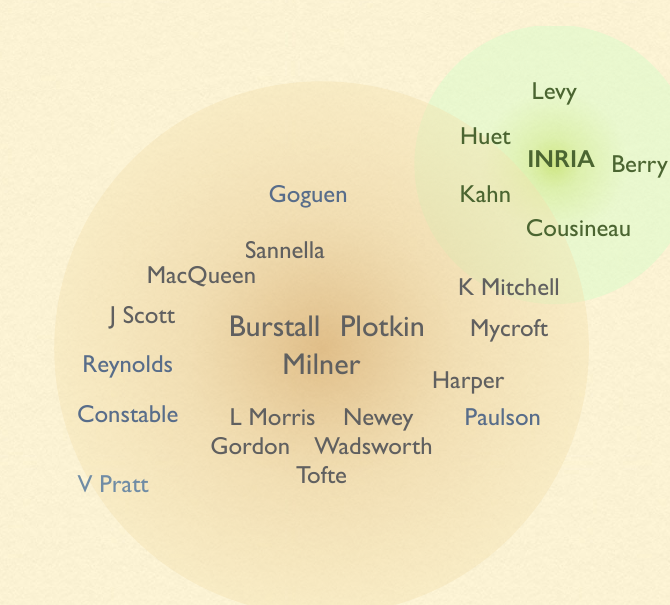
\includegraphics[angle=0,scale=0.7]{two_circles.png}

Самый первый $M\!L$, также известный как $DEC10\ ML$, встраивался в систему $LCF$ как метаязык. Логика Скотта в нём описывалась с помощью объектного языка $PPLAMBDA$. В $M\!L$ поддерживались термы, формулы и теоремы, при этом теоремы являлись абстрактными типами и их конструирование из термов могло происходить только путём применения правил вывода, таким образом в языке не могло появиться неверных теорем. В $LCF$ присутствовала возможность преобразования синтаксического  дерева $M\!L$ в код и наоборот (техники, называемые quotation/antiquotation). Функциональный язык программирования был необходим, чтобы с помощью комбинирования тактик высшего порядка строить новые тактики, а сильная типизация -- чтобы не было обходных способов создать теоремы.

Основные свойства $LCF/ML$:
\begin{itemize}
  \item Основан на $ICW\!IM$.
  \item Вывод типов через милнеровский let-полиморфизм.
  \item Абстрактные типы данных (через ключевое слово abstype).
  \item Тип-сумма и тип-произведение (\verb=t1+t2=, \verb=t1#t2=).
  \item Изменяемые значения через объявление letref (с весьма нетривиальными правилами типизации).
  \item Вложенные кортежи и шаблоны для байндинга списков (pattern-matching).
  \item Условные циклы.
  \item Поддержка ошибочных ситуаций путём передачи строк, которые назывались токенами. Различные виды "ловушек" (обработчиков исключений-токенов): простые, условные и зацикливающиеся.
\end{itemize}

Компилятор для $LCF/ML$ был изначально написан на $LISP$ (вначале на диалекте Standford, потом Rutgers). Код с $M\!L$ транслировался в $LISP$ и интерпретировался, поэтому работал весьма медленно. Парсер\footnote{В русскоязычной литературе также используется термин "синтаксический анализатор".} был основан на приоритетном парсере Вона Пратта (Vaugnan Pratt), который имел следующую особенность: функции-парсеры прикреплялись к отдельно взятым символам, в то время как было бы более естественно использовать разные парсеры для одного и того же символа в зависимости от контекста. Таким образом получалось, что если запятая использовалась для разделения элементов кортежа, то её нельзя было переиспользовать для разделения элементов списка, а если точка с запятой использовалась для разделения элементов списка, то для оператора следования нужно было использовать удвоенную точку с запятой, и т.д.

\subsection{VAX ML (или Cardelli ML)}
В 1980 Лука Карделли начинает работу на собственным диалектом $M\!L$ и его компилятором. К 1981 году он реализовывает его полностью на паскале, включая и сборщик мусора. В данной реализации были следующие нововведения:
\begin{itemize}	
\item Именованные структуры и варианты был основаны на плоткинских лекциях по теории доменов. До этого они не объявлялись явно перед использованием.
\item Комбинаторы для управления вычислениями (declaration combinators):
      \begin{itemize}
	\item and -- одновременно;
	\item enc -- последовательно (enclosing)  ⇒ \verb=d1;d2=;
	\item ins -- локально  ⇒ \verb=local d1 in d2 end=;
	\item rec -- рекурсивно;
	\item with -- для особой формы абстрактных типов (объявления вида \verb=with t ⇔ ty=);
      \end{itemize}
\item Оператор для ссылочного типа (ref type) вместо конструкции letref. А также правила вывода для него: ref, !, :=.
\item Ввод-вывод с помощью потоков.
\item Базовая поддержка модулей с раздельной компиляцией.
\end{itemize}

Компилятор $V\!AX\ ML$ был также реализован в Эдинбурге в 1980-1982 годах, где запускался под операционной системой $V\!AX/V\!MS$. Он также был написан на Паскале, включая библиотеки времени выполнения. Код компилировался в  виртуальную машину $FAM$ (Functional Abstract Machine), которая генерировала код для $V\!AX$ машины из $F\!AM$ кода. В этой реализации впервые поддерживался импорт/экспорт модулей на лету. Данный компилятор вместе с операционной системой продавался пользователям начиная с 1981 года.

Развитие $V\!AX\ ML$ показало, что $M\!L$ может использоваться как язык общего назначения и имеет эффективную реализацию. Это привело к росту количества диалектов $M\!L$ и последующему предложению от Робина Милнера “стандартизовать” $M\!L$ ($Standart\ M\!L$ или $SM\!L$, апрель 1983). Таким образом,  $V\!AX\ M\!L$ являлся непосредственным предшественником $SM\!L$ и тестовой площадкой для ранних экспериментов над дизайном $SM\!L$.

Из самых важных встреч для обсуждения дизайна можно выделить три: состоявшиеся в апреле 1983 года, июне 1984 и мае 1985. 

Так получилось, что большое количество людей собралось в Эдинбурге в апреле 1983, и Бернард Суфрин организовал встречу в гостиной Робина Милнера, где хозяин дома представил своё виденье дизайна языка \cite{milner2}. К данной встрече бы написан первый черновик дизайна и включал в себя лучшие идеи из языков $LCF/M\!L$, $V\!AX\ M\!L$ и $Hope$. 

%Физические участники
%Rod Burstall, Luca Cardelli, Guy Cousineau, Mike Gordon, David MacQueen, Robin Milner, Kevin Mitchell, Alan Mycroft, Larry Paulson, David Rydeheard, Don Sannella, John Scott, Brian Monahan, Stefan Sokolowski
%virtual participants
%Gerard Huet, Peter Mosses, David Schmidt

Название для языка Робин Милнер выбрал сам, надеясь предотвратить длительные споры о названии и дизайне. Но это оказалось ошибкой, потому что такое амбициозное имя в некотором смысле "приклеилось" к $M\!L$ и вводит в заблуждение людей мало знакомых с этой темой.

Основные возможности, заявленные в первом дизайне языка:
\begin{itemize}
\item Формы объявления типов данных, конструкторы в паттернах.
\item Без записей и вариантов (в смысле $V\!AX\ M\!L$).
\item Функциональные выражения с клаузами: \verb=fun v1. e1 | ... | vn. en=.
\item Мономорфные ссылки и равенство.
\item "Локальные" объявления значений вместо специального оператора \verb=ins= из $Cardelli\ M\!L$.
\item Механизм обработки ошибок (escape) с токеном и единая форма обработки (trap) для этого: \verb=e1 trap v1. e1 | ... | vn. En=. Но исключения могли в себе нести только строки.
\end{itemize}
%
%Дальнейшие черновики непосредственно языка:
%\begin{itemize}
%4/83: Changes to proposal for Standard ML, Milner
%6/83: A Proposal for Standard ML (второй черновик), Milner (49 страниц)
%11/83: A Proposal for Standard ML, Milner (27 pages) [“конечный черновки”]
%6/84: Record of the Standard ML Meeting, Edinburgh, 6-8 June 1984
%MacQueen and Milner
%7/84: Standard ML - The Core Language, Milner [changes summary]
%7/84: The Standard ML Core Language, Milner [LFP 84 draft?]
%10/84: The Standard ML Core Language, Milner
%6/85: Report on the Standard ML Meeting, Edinburgh, May 23-25, 1985, 

%9/85: The Standard ML Core Language (Revised), Robin Milner
%\end{itemize}

В те времена ещё не были распространены $email$ и $ARPANET$, поэтому вся переписка велась через почтовое сообщение. Постепенно спецификация стандарта менялась, наращивая небольшие изменения. В июне 1985 года люди собрались во второй раз, называв эту встречу $ML\ Workshop$. Так состоялся первый $ML\ Workshop$, который проводится каждый год по сей день.

По мимо черновиков стандарта самого языка рассматривались предложения по системам ввода-вывода и модулей.

%Other Design Drafts - I/O and Modules
%Stream I/O:
%12/83: Stream Input/Output, Cardelli [Polymorphism 3,1]
%2/85: Proposal for I/O in Standard ML, K. Mitchell and Milner
%6/85: Standard ML Input/Output, Harper [ML Workshop 85]
%Modules:
%8/83: Modules for Standard ML, MacQueen [preliminary, incomplete draft]
%8/84: Modules for Standard ML, MacQueen [LFP 84, Polymorphism]
%10/85: Modules for Standard ML, MacQueen [final draft before Definition]




\subsection{Standard ML (SML 90)}
Работы над формальным описанием языка начались в районе 1986 года. Всего было в Эдинбурге было выпущено три издания стандарта языка. Работы велись преимущественно Робином  Милнером, Робертом Харпером и учеником Робина Милнера Мэдсом Тофтэ.
\begin{itemize}
\item 8/87: The Semantics of Standard ML, издание 1.
\item 8/88: The Definition of Standard ML, издание 2.
\item 5/89: The Definition of Standard ML, издание 3.
\end{itemize}
Финальная версия спецификации языка была выпущена в 1990 году в издательстве MIT Press.

Одним из самых важных нововведений $SML 90$, которое было предложено не в самом начале, была поддержка исключений как расширяемых типов данных: язык был расширен конструкторами исключений и сопоставлением с образцом (pattern matching) исключений в их обработчике. 

Три ранние реализации $Standart\ M\!L$:
\begin{itemize}
\item $Cardelli\ M\!L$ (или $V\!AX\ M\!L$) можно назвать "полустандартным" $M\!L$ -- в нём были поддержанны особенности языка, предложенные в 1983-84 годах.
\item $Edinburgh\ ML$ => $Edinburgh\ SM\!L$.
\item Кэвин Митчелл (Kevin Mitchell), Алан Майкрофт (Alan Mycroft), Джон Скотт (John Scott) и Роберт Харпер (Robert Harper) переписали на $Cardelli\ ML$ компилятор 
$Cardelli\ ML$.
\item Дэйв Мэтьюс (Dave Matthews) реализовал на $SML$ синтаксический анализ для своего языка $PolyML$.
\end{itemize}

Более поздние реализации:
\begin{itemize}
 \item Standart ML of New Jersey ($SML/N\!J$);
 \item MLKit;
 \item Moscow ML;
 \item MLton.
\end{itemize}

\subsection{Главные идеи в  Standard ML ‘90}
\begin{itemize}
\item Let-полиморфизм, вывод типов, наиболее общие (principal) типы: статьи Макса Ньюмана (1940е), Хаскелла Карри (1969) \cite{curry1}, Рождера Хиндли (1969) \cite{hindley1}, Робина Милнера\cite{milner1}.
\item Алгебраические типы данных и функции с клаузами, разбор случаев с помощью сопоставления с образцом (заимстовано из языка $Hope$).
\item Модули и их сигнатуры, функторы, спецификации разделения данных и генеративные структуры (“strong structure sharing”): структуры  с  некоторой статической уникальной идентичностью, которые  можно было сравнивать, т.е. на этапе компиляции проверять, что структуры равны. У этой особенности языка получилась очень сложная семантика, потому она не стала особо популярной.
\item Исключения как расширяемый тип данных.
\item Поддержка изменяемых значений (а именно ссылочных типов -- ref types) используя  понятие "императивных переменных типа" (imperative type variables) привела к некоторому количеству сложностей в языке. Было написано большое количество статей на тему того как улучшить данных подход и почему от него стоит отказаться.
\end{itemize}

Эволюция алгебраических типов данных:
\begin{enumerate}
\item Неформальные описания данных, использованные в $I\!SW\!I\!M$.
\item Формальное развитие этих методов в работе Питера Лондина и Рода Берстолла “Programs and Their Proofs: An Algebraic Approach” \cite{laundin5} (полуформально описаны).
\item “Игрушечный” язык Берстаола $N\!P\!L$.
\item В языке $Hope$ более-менее полно сформировались и были заимствованы оттуда в $Standart\ ML$.
\end{enumerate}



%Картинка
%\begin{verbatim}
%datatype AE = ID of identifier
%            | LAMBDA of {bv: identifier, body : AE}
%            | COMB of {rator : AE, rand : AE}
%\end{verbatim}

\subsection{Ошибки в процессе дизайна}
"Замораживание” формального описания языка в виде книги оказалось плохой идеей. Если язык программирования обретает реализацию и начинает использоваться, то его спецификацию необходимо поддерживать, а также (весьма осторожно) позволять языку изменяться. Описание должно быть открытым, но при этом очень аккуратно поддерживаемым.
Возникновение этой проблемы связано со степенью участия Робина  Милнера в проекте. Он был весьма занятым человеком, его основными проектами в то время были $CCS$ (исчисление взаимодействующих систем, Calculus of Communicating Systems) и пи-исчисление. Ему хотелось дойти до состояния, когда он может передать рукопись в издательство MIT  и перестать думать об этом проекте. Для своих целей он не планировал реализовывать, поддерживать и даже использовать этот язык. Следует помнить, что в те времена не существовало $WWW$, так что не было возможности выложить описание в онлайн.

Выпущенная книга про $SML’90$ имела очень короткое (2-3 страницы) приложение про “основы”, что по сути являлось стандартной библиотекой типов и функций. Список был очень короткий и состоял только из 43х пунктов, таким образом, каждый кто реализовывал $SM\!L$ должен был расширять этот перечень, и каждая реализация расширяла этот список несовместимым друг с другом способом. Процесс "устаканивания" занял довольно длительное время, до тех пор пока Джон Реппи (John Reppy) не взялся за эту проблему и не создал “SML Basis Library”. Однако, эта работа вышла в свет лишь спустя несколько лет после $SML‘97$.

% там кроме Reppy был Gasner но лень искать кто это.

\subsection{Развитие языка в 1990е годы}
В 1997 году институт Ньютона (Isaac Newton Institute for Mathematical Sciences), а именно программа по исследованию семантики вычислений собрала Робина Милнера, Роберта Харпера, Макса Тофтэ и Дэйва МакКуина в Кембридже, где они начали работу по переработке описания языка $Standart\ M\!L$ \cite{sml97}. Вот значимые изменения:

\begin{itemize}
\item Сокращения типов в сигнатурах (реализовано в $SML/N\!J$ 0.93 и в $Caml\ Special\ Light$ \cite{leroy1}).
\item Непрозрачное сравнение сигнатур.
\item Слабое разделение сигнатур (подразумевает собой только равенство типов).
\item Полиморфизм значений: уход от императивных типовых переменных, переход к ограничению полиморфизма значений (value restriction).
\item Клонирование типов данных.
\end{itemize}
%Также хотели выкинуть equality types, но Милнер застеснялся.

\subsection{ML2000}
Серия встреч между 1993 и 2000 годами была посвящена идее создания $M\!L$ “следующего поколения”, но консенсус так и не был найден в основном из-за не согласия участников по поводу добавления объектно-ориентированных возможностей в язык. В то время уже существовали языки со своей собственной реализацией объектов такие как $OCaml$, а также язык $Moby$ за авторством Джона Рэппи (John Reppy) и Кэтлин Фишер (Kathleen Fisher). Основные предлагаемые изменения в языке были опубликованы в Principles and Preliminary Design of $ML2000$ \cite{ML2000}. 


\section{OCaml}
Изначально, “Caml” являлся акронимом для Categorical Abstract Machine Language ($CAM$) -- языком для Категориальной Абстрактной Машины. Имя языка является слиянием названия машины и семейства языков, которому он принадлежит. Название $Caml$ сохранилось на протяжении всей эволюции языка, несмотря на то, что современная реализация не имеет никакого отношения к $CAM$.

$Caml$ был создан в исследовательской группой $Formel$ из $INRIA$, которой руководил Жерар Уэ (Gérard Huet). Его развитие продолжалось в исследовательских группах $Cristal$, и современной $Gallium$.

\subsection{Истоки}
Лаборатория $Formel$ начала интересоваться языком $M\!L$ в начале 80х годов. В те времена $M\!L$ использовался в $LCF$, а сам $LCF$ был написан частично на $LISP$, частично на $M\!L$. В $Formel$ использовались несколько операционных систем ($Multics$, $Berkeley\ Unix\ on\ Vax$, $Symbolics$), поэтому Жерар Уэ решил создать реализацию $M\!L$, которая будет совместима одновременно с несколькими компиляторами $LISP$ ($MacLisp$, $FranzLisp$, $LeLisp$, $ZetaLisp$). В работу были вовлечены Гай Кузино (Guy Cousineau) и Ларри Паульсон (Larry Paulson). В придачу к созданию компилятора была существенна увеличена производительность языка.

Гай Кузино, следуя идеям Робина Милнера, также добавил в язык сопоставление с образцом и алгебраические типы данных, которые он заимствовал из языка $Hope$, спроектированного Родом Берстоллом и Дэйвом МакКуином. Некоторое время эта реализация называлась "Le ML", но это название не прижилось. 
%\b{It was used by Larry Paulson to develop Cambridge LCF and by Mike Gordon for the first version of HOL, as recalled in Gordon's short history of HOL}.

Около 1984 года, когда Робин Милнер предложил формальную спецификацию $M\!L$, а Лука Карделли уже имел эффективную реализацию $M\!L$ для $FAM$, Пьер-Луи Курье разработал исчисление категориальных комбинаторов, а также соответствие между ними и лямбда-исчислением. Это наблюдение использовал Гай Кузино для реализации эффективного способа компиляции в $M\!L$. Этот способ был близок к тому, что был использован в $Edinburgh\ M\!L$, но мог быть формально описан, доказан и по-простому оптимизирован. Это привело к появлению Категориальной Абстрактной Машины. 

Таким образом Гаю Кузино была необходима новая реализация, основанная на $CAM$. Однако, в итоге получился не $Standart ML$, а $Caml$. Почему? Главной причиной для разработки $Caml$ было то, что он использовался в лаборатории $Formel$ как основной язык для внутренней разработки. Также он использовался для разработки системы $Coq$, которая после появления выпускной работы Тьери Кокана (Thierry Coquand) стала основным направлений исследований в $Formel$. Группа не приняля  "стандартного" синтаксиса, потому что он мог помешать адаптации языка под текущие нужды. В частности, Филипп Лё Шенадэ (Philippe Le Chenadec) и Мишель Мони (Michel Mauny) разработали утилиты для манипуляции синтаксисом, которые оказались весьма полезными и были интегрированы в $Caml$. Обсуждение изменений, которые выглядели полезными, с разработчиками $Standart ML$ внесло бы чересчур большую задержку в работу. Более того, философия ведения разработки противоречила "стандартному" языку, где не предполагалось слишком быстрых изменений. Таким образом, все существенные улучшения, которые появлялись в $Standart\ ML$ и $Edinburgh\ ML$ вручную переносились в $Caml$.

\subsection{Первая реализация}
Первая реализация $Caml$ появилась в 1987 году и продолжала своё развитие до 1992 года. Она были сделана в основном Аскандером Суарезом (Ascander Suarez). После того, как он покинул лабораторию в 1988 году, Пьер Вей (Pierre Weis) и Мишель Мони (Michel Mauny) занимались развитием и поддержкой до 1992 года. Эта реализация компилировала $Caml$ в  $LLM3$, виртуальную машину системы $Le\ Lisp$. Гай Кузино скромно вспоминает: "Я должен признать, что когда начиналась разработка $Caml$, я имел весьма небольшой опыт в языках программирования. То, что мы взяли за основу систему $Le\ Lisp$ и её механизмы по выделению памяти и сборке мусора, сэкономило нам много времени, но не позволяло получить высокой производительности. Модель $CAM$ позволяла быстро конструировать замыкания и разделять области видимости, но с доступом к окружению и применением оптимизаций были сложности. Также она могла порождать утечки памяти, так как ненужные значения сохранялись в замыканиях. Также, я не сразу осознал, что более важным является хорошая производительность не-функциональных программ, чем полностью  написанных в функциональном стиле. Также я недооценил важности портируемости языка на другие платформы и открытости модели разработки. Несмотря на эти неувязки, ответственность за которых я беру на себя, Аскандер, Пьер и Мишель выполнили великолепную работу."


\subsection{Caml Light}
В 1990 и 1991 годах Завье Леруа (Xavier Leroy) спроектировал абсолютно новую реализацию $Caml$, в основе которой лежал интерпретатор байт кода, написанный на $C$. А Дамьен Долигэ (Damien Doligez) спроектировал великолепную систему управления памятью. Эта новая реализация, получившая название $Caml\ Light$, была легко портируемой и запускалась на таких небольших домашних компьютерах как Macintosh и PC. Она заменила старую реализацию $Caml$ и привела к росту популярности $Caml$ в системах высшего образования и научно-исследовательских лабораториях. Поддержка потоков данных и технологии синтаксического анализа (благодаря Мишелю Мони) позволила команде $Formel$ создать необычные системы управления синтаксисом. 

\subsection{Caml Special Light}
В 1995 году Завье Леруа анонсировал $Caml\ Special\ Light$, который улучшил $Caml\ Light$ в нескольких аспектах. Во-первых, это оптимизирующий компилятор в машинный код, который был сравним или превосходил производительность лучших на тот момент компиляторов функциональных языков и позволил $Caml$ соревноваться в производительности с  такими языками как $C\!+\!+$. Во-вторых, в $Caml\ Special\ Light$ была высокоуровневая система модулей, спроектированная Завье Леруа на основе системы модулей в $S\!M\!L$. Эта система предлагала богатые возможности абстракции и программирования в целом. 
% "в целом"?

\subsection{Objective Caml}
Системы типов и системы вывода типов для объектно-ориентированных языков были популярной темой для исследования в начале 1990х годов. Дидье Рэми (Didier Rémy), к которому позднее присоединился Жером Вульон (Jérôme Vouillon), разработал элегантную и выразительную систему типов для объектов и классов. Реализация была интегрирована в 
$Caml\ Special\ Light$, что привело к появлению в 1996 году реализации языка $Objective\ Caml$, который был переименован в $OCaml$ в 2011 году. Он является первым языком, который сочетает выразительность объектно-ориентированного программирования со статической типизацией в стиле $M\!L$ и выводом типов.  Он поддерживает большинство современных идиом объектно-ориентированного программирования (параметрические классы, бинарные методы, специализация) статически и типобезопасно, в то время как в других языках ($C\!+\!+$ и $Java$) это приводит к противоречивости системы типов или необходимости проверок во время выполнения.

В 2000 году Жак Гариг (Jacques Garrigue) расширил $Objective\ Caml$ некоторыми возможностями, над которыми экспериментировал в диалекте $Objective\ Label$. Среди них полиморфные методы, именованные и опциональные параметры функций, полиморфные варианты.
% полиморфные методы ?????
%In 2000, Jacques Garrigue extended Objective Caml with several new features, which he had been experimenting with for a few years in the Objective Label dialect of Objective Caml. Among these features were polymorphic methods, labeled and optional function arguments, and polymorphic variants.

Расцвет OCaml пришелся на конец 1990х, когда он начал набирать популярность и привлекать существенное количество пользователей.
%The rise of OCaml
%Since the late 1990's, OCaml has been steadily gaining in popularity and attracted a significant user base. In addition to impressive programs developed in %OCaml, the user community also contributed many high-quality libraries, frameworks and tools in areas ranging from graphical user interfaces and database %bindings to Web and network programming, cross-language interoperability and static program analysis. In parallel, the core OCaml development team actively %maintains the base system, improving the quality of the implementation and porting it to the latest architectures and systems. As lead developer of OCaml, %Chair of the Caml Consortium and Owner of OCaml.org, Xavier is considered to be benevolent dictator for life (BDFL) of the OCaml language.

%\subsection{Некоторые ближайшие родственники}
%In addition to these mainstream versions of Caml, one should mention many related compilers. Michel Mauny and Daniel de Rauglaudre designed Chamau, which %offers unique syntax manipulation facilities which are now offered in the Camlp4 pre-processor for OCaml.
%Manuel Serrano and Pierre Weis created BIGLOO. Régis Cridlig made Camlot. Jean Goubault-Larrecq wrote HimML, which features implicit hash-consing and %efficient operations on sets and maps. Emmanuel Chailloux published CeML. In the Para team, Francis Dupont implemented Caml for parallel machines, while %Luc Maranget built Gaml, a compiler for a lazy functional programming language.

В 1996 году Гай Кузино писал: "Конечно, история $Caml$ могла быть более линейной. Однако, методом проб и ошибок, во Франции появился функциональный язык программирования достаточно гибкий, портируемый и обладающий хорошей производительностью."

\section{Заключение}
В рамках реферата была рассмотрена история появления основных языков семейства $M\!L$: $Standart\ M\!L$ и $OCaml$, был рассмотрен контекст и нужды, для которых эти языки создавались, очерчены родственные связи этих языков с современными императивными языками программирования. Также была предпринята попытка проанализировать ошибки, совершенные при проектировании языков. Были обозначены цели, к которым надо стремиться при проектировании нового языка программирования.

Развитие языков функционального программирования и, в частности, $M\!L$, является перспективной темой для проведения исследований, так как наличие формальной семантики у этих языков, и, как следствие, появление систем-помощников в доказательстве теорем, позволяет создавать программы с формально доказуемой корректностью. А доказанная корректность является сама по себе очень полезным свойством для практического программирования, в частности, при разработке высоконадёжных систем (в ядреной энергертике, космической отрасли, медицине и т.д.).

\newpage
\section{Литература}
\begin{thebibliography}{9}
  \bibitem{russel1}
    A.N. Whitehead, B. Russell Principia mathematica 1 (1 ed.), Cambridge: Cambridge University Press, 1910.
  \bibitem{bcpl1}
    M. Richards, The BCPL Reference Manual, Memorandum M-352, Project MAC, Cambridge, MA, USA, 1967.
  \bibitem{strachey1}
    C. Strachey. Fundamental concepts in programming languages, Lecture Notes, International Summer School in Computer Programming, Copenhagen, 1967.
  \bibitem{strachey2}    
    C. Strachey. Time sharing in large fast computers, UNESCO Conference on Information Processing, Paris, 1959. 
  \bibitem{scott1}
    D. Scott, C. Strachey. Toward a mathematical semantics for computer languages, Oxford Programming Research Group Technical Monograph, PRG-6, 1971.
  \bibitem{laundin1}
    Peter J. Landin. The mechanical evaluation of expressions, The Computer Journal, British Computer Society 6 (4): pp. 308–320, 1964.
  \bibitem{laundin2}
    Peter J. Landin. Correspondence between ALGOL 60 and Church's Lambda-notation: part I, Communications of the ACM 8 (2): pp. 89–101, 1965.
  \bibitem{laundin3}
    Peter J. Landin. "A Generalization of Jumps and Labels, UNIVAC Systems Programming Research (technical report).
  \bibitem{laundin4}
    Peter J. Landin. The next 700 programming languages, Communications of the ACM 9 (3): 157–166, 1966.
  \bibitem{laundin5}
    R. M. Burnstall, Peter J. Landin. Programs and their proofs: an algebraic approach, Machine Intelligence 4, 1969.
  \bibitem{hope1}
    R. M. Burstall, D. B. MacQueen, D.T. Sannella. Hope: An Experimental Applicative Language, Conference Record of the 1980 LISP Conference, Stanford University, pp. 136-143, 1980.
  \bibitem{npl1}
    J. Darlington, R. Burnstall, . "Program Transformation and Synthesis: Present Capabilities". Research Report No. 77/43, Dept. of Computing and Control, Imperial College of Science and Technology, 1977.
  \bibitem{ML2000}
     The ML2000 Working Group. Principles and a Preliminary Design for ML2000, 1999.
  \bibitem{leroy1}
     X.Leroy. Manifest types, modules, and separate compilation, Proc. 21st Symp. Principles of Programming Languages, pp. 109–122, 1994.
  \bibitem{hindley1}
     J. R. Hindley, The principal type scheme of an object in combinatory logic, Transactions of the American Mathematical Society (American Mathematical Society) 146: 29–60, 1969.
  \bibitem{curry1}
     H. B. Curry. A Theory of Formal Deducibility, J. Symbolic Logic Volume 34, Issue 1, 1969.
  \bibitem{milner1}
     R. Milner. A theory of type polymorphism in programming, Journal of Computer and System Sciences, 17:348-375, 1978.
  \bibitem{milner2}
     R. Milner. A proposal for standard ML, LFP '84 Proceedings of the 1984 ACM Symposium on LISP and functional programming, 1984
  \bibitem{sml97}
     R. Milner, M. Tofte, R. Harper and D. MacQueen, The Definition of Standard ML (Revised), MIT Press, 1997.
  \bibitem{macqueen1}
     D. MacQueen, The history of Standart ML: ideas, principles, culture, ML Family Workshop, 2015.
\end{thebibliography}

\end{document}

